%!TEX TS-program = pdflatex
\documentclass{robinthesisdraft}
\usepackage{robincs,thesisdefs,xr,tikz,prooftree}
\externaldocument[Bicats:]{bicats}
\externaldocument[MonBicats:]{mon-bicats}

\title{A Language for Gray Monoids}
\begin{document}
\maketitle
%
\section{The problem}
Even with the help of the coherence theorem, it can be extremely
tedious to prove even simple facts about pseudomonoids. The problem
is essentially notational rather than mathematical: in an ordinary
category, we can use commutative diagrams to establish equations
between arrows. It is almost always easier to understand a diagram
than an explicit sequence of equalities between expressions, because
\begin{itemize}
\item The types of the arrows are clear from the diagram.
\item The diagram abstracts away from certain details of the proof:
	if two equations could be applied in either order, the diagram
	does not have to choose an order arbitrarily.
\item The global structure of the whole argument can be seen at a glance.
\end{itemize}
In a bicategory, to prove an equation between 2-cells by similar
means, we should need three-dimensional diagrams. This poses
practical problems -- paper is two-dimensional -- and also requires
the reader to visualise a three-dimensional structure, something
that most humans do not find easy. This technique has sometimes
been attempted nonetheless: by \citet[][Section~3.4]{LackThesis},
for example.
%
The more usual alternative is to use a sequence of equations
between string or pasting diagrams. As well as using a lot
of paper, such proofs are often difficult to follow. (We do
find ourselves obliged to resort to this technique in some
places where the techniques of this chapter do not apply.)

The purpose of this chapter is to show how these notational
difficulties may, in some cases, be overcome by using a formal
language to specify 1-cells, 2-cells, and equations between 2-cells
in a Gray monoid. The syntax of the language is designed in such
a way that a proof using the language closely resembles a proof
using categories, functors and natural transformations in the usual
way. In other words, provided that one uses only admissible techniques,
a proof in the Gray monoid $\Cat$ may be reinterpreted
as a general proof that applies to any Gray monoid. In particular,
we shall be able to prove various general facts about pseudomonoids
simply by reusing the usual proof of the corresponding fact for
monoidal categories.

The formal language is not completely general. The fundamental
restriction is that it may only be used to talk about theories
whose 1-cells are of the form
\[
	A_{1}\tn\cdots\tn A_{n} \to B.
\]
In particular, the braiding on a braided Gray monoid is not of this
form, and we will be unable to use this language to prove facts about
structures that interact with the braiding, such as the braiding of
a braided pseudomonoid. So we are really describing an internal
language for category-enriched multicategories, rather than for
general Gray monoids. It is, however, more than adequate for the
purpose of describing and proving results about pseudomonoids.
%
This restriction is not, strictly speaking, essential; but it
significantly simplifies the language. In particular, it
insulates us from the inconvenient fact that the interchange
law of a Gray monoid does not hold on the nose.

The language itself is rather trivial, and its formal description
is entirely routine. That is the point, in a way. The obvious%
\footnote{Of course, they seem obvious only as a result of decades
	of work on logic and type theory!}
definitions do indeed work, and nothing surprising happens,
the end result of which is a convenient language for expressing proofs.

\section{The language}
The language is used to prove equations between 2-cells that hold in
every model of a given theory. As
suggested above, we think of a model of a theory as being a category-enriched
multicategory. 
% Since this perspective is used only to provide
% intuition, and not in any technical capacity, we shall not pause
% to give a formal definition of enriched multicategories: the
% interested reader could consult \citet[][p.~39 and Example~6.8.3]{LeinsterBook}.
In fact we only define the interpretation in a Gray monoid, since
to formally introduce enriched multicategories here would be a
needless distraction.
%
We require the theory to be presented as a collection
of objects, (multi-)1-cells, 2-cells and equations between 2-cells.

A \emph{theory} $\T$ consists of:
\begin{itemize}
	\item A set $\T_{0}$ of \emph{objects},
	\item For every non-empty sequence $A_{1}, \ldots, A_{n}, B$ of
		elements of $T_{0}$,
		a set $\T(A_{1},\ldots,A_{n};B)$
		of \emph{1-cells} $(A_{1}, \dots, A_{n})\to B$.
	\item Sets of 2-cells and equations, as described below.
\end{itemize}
Before we attempt a formal description of the 2-cells and equations,
we shall introduce the part of the language that describes 1-cells.

A 1-cell will be described by a \emph{1-cell sequent}: suppose
we are considering a theory with objects $\A, \CB, \C$ and
1-cells $f: (\A,\CB)\to\C$ and $g:\C\to\C$. Then the arrow
\[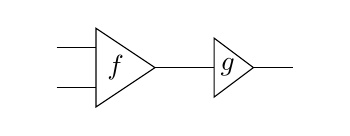
\begin{tikzpicture}[scale=0.25]
	\draw (0,-2) -- (0,2) -- (3,0) -- cycle ;
		\node at (1,0) {$f$} ;
	\node at (-3,1)  {$\A$}  ; \draw (-2,1) -- (0,1) ;
	\node at (-3,-1) {$\CB$} ; \draw (-2,-1) -- (0,-1) ;
	\draw (3,0) -- (6,0)
		node[pos=0.5,auto] {$\C$} ;
	\draw (6,-1.5) -- (6,1.5) -- (8,0) -- cycle ;
		\node at (6.7,0) {$g$} ;
	\draw (8,0) -- (10,0) ;
		\node at (11,0) {$\D$} ;
\end{tikzpicture}\]
might be represented by the sequent
\[
	A\in\A, B\in\CB \proves g(f(A,B)) \in \D.
\]
The names in the context -- to the left of the turnstile -- should
be regarded as bound, so for example the sequent
\[
	X\in\A, Y\in\CB \proves g(f(X,Y)) \in \D
\]
is equivalent to the one above, modulo the renaming of bound
variables, and represents the same 1-cell. (We assume
throughout that we have some infinite set of names
on which to draw. Names here will be represented
by upper-case italic letters.)
Formally, the derivation rules for 1-cell sequents are
as follows:
\begin{itemize}
\item For every $\C\in\T_{0}$,
\[
	\begin{prooftree}
		\justifies A\in\C \proves A\in\C \using (\C)
	\end{prooftree}
\]
\item For every $f\in\T(\A_{1},\dots,\A_{n}; \CB)$,
\[
	\begin{prooftree}
		\Gamma_{1}\proves \alpha_{1}\in \A_{1}
		\quad
		\cdots
		\quad
		\Gamma_{n}\proves \alpha_{n}\in \A_{n}
		\justifies
		\Gamma_{1},\dots,\Gamma_{n} \proves f(\A_{1},\dots,\A_{n})\in\CB
		\using f(\bullet)
	\end{prooftree}
\]
where the names in the $\Gamma_{i}$ are assumed pairwise disjoint.
\end{itemize}
So a 1-cell sequent is simply a formal composite of formal 1-cells.
It is clear by induction that every derivable 1-cell sequent has a unique
derivation.

Now we can define the 2-cells of $\T$. In addition to the
objects and 1-cells, we have:
for every pair $\Gamma\proves\alpha\in\A$, $\Gamma\proves\beta\in\CB$
of derivable 1-cell sequents, a set $\T^{\Gamma}_{\A}[\alpha,\beta]$
of 2-cells. Of course, we take these to be invariant under renaming,
so if $\sigma$ is a permutation of the set of names then we require
\[
	\T^{\Gamma^{\sigma}}_{\A}[\alpha^{\sigma},\beta^{\sigma}] = \T^{\Gamma}_{\A}[\alpha,\beta].
\]
%
A 2-cell sequent is of the form $\Gamma\proves \phi: \alpha\to\beta \in\C$.
The derivation rules for 2-cell sequents are:
\begin{itemize}
% \item The identity rule:
% 	\[\begin{prooftree}
% 		\Gamma\proves \alpha\in\A
% 		\justifies
% 		\Gamma\proves 1_{\alpha}: \alpha\to\alpha\in\A
% 		\using 1
% 	\end{prooftree}\]
% 	(Actually we won't ever need the identity rule, but
% 	it's a perfectly good rule, so we include it anyway.)
\item The axiom rule: for every $t\in \T^{\Gamma}_{\A}[\alpha,\beta]$,
	\[\begin{prooftree}
		\justifies
		\Gamma\proves t_{[\Gamma]}: \alpha\to\beta\in\A
		\using (t)
	\end{prooftree}\]
	where $[\Gamma]$ denotes the list of names from the
	environment $\Gamma$.
\item The composition rule:
\[\begin{prooftree}
	\Gamma\proves \phi: \beta\to\gamma \in\A
	\quad
	\Gamma\proves \psi: \alpha\to\beta \in\A
	\justifies
	\Gamma\proves \phi\cdot\psi: \alpha\to\gamma \in\A
\end{prooftree}\]
\item The 1-cell application rule: for every
	
\end{itemize}
We could also include a rule allowing the introduction of
identity arrows. Since we don't need such a rule, and
including one would require some additional equations below,
we have chosen to omit it here.

The final ingredient that we need to complete our description
of $\T$ is a set $\T_{=}$ of equations between 2-cells.
Formally, we could declare that $\T_{=}$ is a set of tuples
$(\Gamma,\alpha,\beta,\phi,\psi)$, where 
$\Gamma\proves\phi:\alpha\to\beta\in\A$ and
$\Gamma\proves\psi:\alpha\to\beta\in\A$ are derivable
2-cell sequents.
%
We must of course require $\T_{=}$ to be invariant under renaming,
again.

The derivation rules for equations are:
\begin{itemize}
	\item There are three rules expressing
	the fact that any equality worth the name should be
	reflexive, symmetric, and transitive. In detail: for
	every derivable 2-cell sequent
	$\Gamma\proves\phi:\alpha\to\beta\in\A$, we have
	reflexivity:
	\[\begin{prooftree}
		\justifies
		\phi=\phi:\alpha\to\beta\in\A
		\using=_{r}
	\end{prooftree}\]
	symmetry:
	\[\begin{prooftree}
		\phi=\psi:\alpha\to\beta\in\A
		\justifies
		\psi=\phi:\alpha\to\beta\in\A
		\using=_{s}
	\end{prooftree}\]
	and transitivity:
	\[\begin{prooftree}
		\psi=\gamma:\alpha\to\beta\in\A
		\quad
		\phi=\psi:\alpha\to\beta\in\A
		\justifies
		\phi=\gamma:\alpha\to\beta\in\A
		\using=_{t}
	\end{prooftree}\]
	\item The axiom rule: for every
	$(\Gamma,\alpha,\beta,\phi,\psi)\in\T_{=}$, we have
	\[\begin{prooftree}
		\justifies
		\Gamma\proves\phi=\psi: \alpha\to\beta
		\using\phi=\psi
	\end{prooftree}\]
	\item The naturality rule:
	XXXX this one is the hardest to express!
	\item The functoriality rule:
	
	\item And the composition rule:
\end{itemize}


\section{Interpretation}
To interpret these sequents in a target Gray monoid $\B$, we need
an interpretation of $\T$. An interpretation
$v:\T\to\B$ consists of:
\begin{itemize}
	\item for every $\A\in\T_{0}$, an object $v(\A)$ in $\B$;
	\item for every $f\in\T(\A_{1},\dots,\A_{n};\CB)$, a 1-cell
	\[
		v(f): v(\A_{1})\tn\cdots v(\A_{n})\to v(\CB);
	\]
	in $\B$.
\end{itemize}
%
The semantic interpretation $\llbracket-\rrbracket_{v}$ of a 1-cell
sequent is defined by induction over its derivation:
\begin{itemize}
\item $\Bigl\llbracket	\begin{prooftree}
	\justifies A\in\C \proves A\in\C \using (\C)
\end{prooftree} \Bigr\rrbracket_{v} = 1_{v(\C)}$,
\item $\left\llbracket\begin{prooftree}
		\[[\pi_{1}]\justifies\Gamma_{1}\proves \alpha_{1}\in \A_{1}\]
		\quad\cdots\quad
		\[[\pi_{n}]\justifies\Gamma_{n}\proves \alpha_{n}\in \A_{n}\]
		\justifies
		\Gamma_{1},\dots,\Gamma_{n} \proves f(\A_{1},\dots,\A_{n})\in\CB
		\using f(\bullet)
	\end{prooftree}\right\rrbracket_{v}$
	\newline\vskip1ex\strut\hfil$= v(f)\o\Bigl(
	\biggl\llbracket\begin{prooftree}
		[\pi_{1}]\justifies\Gamma_{1}\proves \alpha_{1}\in \A_{1}
	\end{prooftree}\biggr\rrbracket_{v}
	\tn\cdots\tn
	\biggl\llbracket\begin{prooftree}
		[\pi_{n}]\justifies\Gamma_{n}\proves \alpha_{n}\in \A_{n}
	\end{prooftree}\Big\rrbracket_{v}
	\Bigr)$.
\end{itemize}

\section{Soundness}

\bibliography{cs}
\end{document}